% !TeX spellcheck = en_US
\addscenariosection{1}{Cooperative scenario}{Sentinels}{\images/sentinel.png}

\begin{multicols*}{2}

\textbf{Author:} silence70011

\textbf{Source:} \href{https://discord.com/channels/740870068178649108/1233112440322002964/1233112440322002964}{Archon Studio Discord}

\textit{There is a world beyond this world, and it is filled with beasts and monsters, barely held captive by a formation of four sacred Obelisks.
  But the protection of the stones is weakening, and a breach is imminent.
  When it happens, only you and your ally stand between the hordes and the total devastation of these lands.
}

\subsection*{\MakeUppercase{Scenario Length}}

This scenario is played over 12 rounds.

\subsection*{\MakeUppercase{Player Setup}}

\textbf{Player Count:} 2

\textbf{Starting Resources:}\par
\resources{10}{2}{1}

\textbf{Starting Income:}\par
\resources{10}{2}{1}

\textbf{Starting Units:}
\begin{itemize}
  \item A Pack of \svg{bronze} units with the \textit{lowest} recruitment cost.
  \item A Few \svg{bronze} units with the \textit{highest} recruitment cost.
\end{itemize}

\textbf{Town Buildings:} \svg{bronze} Dwelling, Citadel

\textbf{Map tile Pool:} Each player takes 1 random Near (IV-V) Map tile and 1 random Far (II-III) Map tile.

\textbf{Additional Bonus:} Search (2) the Artifact Deck

\subsection*{\MakeUppercase{Map Setup}}

Take the following Map tiles and set them up as shown in the scenario map layout:

\textbf{2 × Starting (I) Map tile}
\begin{itemize}
  \item Starting Tiles of your chosen factions.
  \item Ignore their yellow borders.
\end{itemize}

\textbf{4 × Far (II-III) Map tile}

\textbf{4 × Near (IV-V) Map tile}
\begin{itemize}
  \item All Near Map tiles must have Obelisks.
\end{itemize}

\subsection*{\MakeUppercase{Victory Conditions}}

Defeat all invading armies.

\subsection*{\MakeUppercase{Defeat Conditions}}

There is an undefeated enemy army left at the end of Round 12.

One of your towns is captured or a main hero is defeated in battle (retreat doesn't count).

\subsection*{\MakeUppercase{Timed Events}}

\textbf{6$^{th}$ and 9$^{th}$ Rounds:}
\begin{itemize}
  \item Remove black cubes from windmills, water wheels, and mystical gardens.
\end{itemize}

\textbf{6$^{th}$-10$^{th}$ Rounds:}
\begin{itemize}
  \item Spawn an enemy army according to the rules below.
\end{itemize}

\subsection*{\MakeUppercase{Additional Rules}}

\begin{itemize}
  \item Players can trade resources when one of the active player's heroes visits a trading post or stands on a field adjacent to an allied hero.
  \item The hero who defeats an enemy army gains 2 \svg{experience}.
    The winning player rolls two Treasure Dice and resolves one of them.
\end{itemize}

\subsection*{\MakeUppercase{Enemy Spawning\\and Movement}}

\begin{itemize}
  \item Enemy armies spawn on a random Obelisk field (use hero miniatures of factions not in play).
  \item Determine which Obelisk field by rolling 2 Attack Dice:
  \begin{itemize}
    \item First die: --1 west, +1 east, 0 reroll
    \item Second die: --1 north, +1 south, 0 reroll
  \end{itemize}
  \item For more equal distribution, in Rounds 7 and 9, the enemy spawns on the opposite side than in the previous round.
    Rounds 8 and 10 are all random.
  \item If the tile to spawn an enemy on isn't discovered yet, flip it over and orient it as preferred.
  \item If there is a hero on the field where the enemy spawns, a fight is initiated immediately.
  \item Enemy armies move at the end of every turn, starting with the same turn they spawned.
  \item Enemy armies have 3 Movement Points per round.
  \item Enemy armies move as described in the rulebook (p. 33), but instead of capturing, they destroy everything in their way.
    Place black cubes on any field they pass and treat them as empty from that point.
  \item If an enemy's movement could go different ways, the players decide which way to go.
\end{itemize}


\subsection*{\MakeUppercase{Combat with\\Enemy Armies}}

\begin{itemize}
  \item During a battle with an enemy army, a hero can retreat every time a friendly unit is about to activate.
    A retreating main hero loses all remaining Movement Points and is returned to an allied town or settlement of their choice, keeping all remaining units.
  \item Retreating secondary heroes are removed from the game, but remaining units are kept.
  \item Killed enemy units do not respawn.
\end{itemize}

\subsection*{\MakeUppercase{Boss Army}}

\begin{itemize}
  \item On Round 10, a Boss Army spawns and is different from previous armies because it gets reinforced from a fixed pool of neutral units (reinforcement pool = number in brackets in the table below).
  \item At the beginning of the 2$^{nd}$ combat round and every following round, 2 units reinforce the remaining army from the shuffled reinforcement pool (up to the maximum of 5 units) to continue the fight until either the player retreats or every neutral unit from the reinforcement pool is killed. \textit{If the number of enemy units at the beginning of a round is 1 or lower, draw up to a total of 4 units (i.e., there are always 4 or 5 enemy units on the board after reinforcing, if available).}
  \item Place the reinforcing units on the enemy base line starting from the left with the lowest initiative (\svg{unit_ranged} units first). If necessary, continue on the next line (in the same order).
  \item When a player retreats, the enemy army draws up to the ``minimum'' of 4 units and takes these as starting units to the next fight.
\end{itemize}

\end{multicols*}

\hommtable[]{18}{
  \centering
  \medskip
  \textbf{Strength of Enemy Armies}\\
  \bigskip

  \newcommand{\bronze}[0]{\svg[12]{bronze}}
  \newcommand{\silver}[0]{\svg[12]{silver}}
  \newcommand{\golden}[0]{\svg[12]{golden}}
  \newcommand{\azure}[0]{\svg[12]{azure}}

  \begin{tabularx}{\linewidth}{p{0.15\linewidth}XXXX} & \darkcell{Rounds 6 + 7} & \darkcell{Rounds 8 + 9} & \darkcell{Round 10}\\
  \darkcell[1.4]{Easy}
    & \lightcell[1.4]{\bronze \silver \silver \silver \golden}
    & \lightcell[1.4]{\silver \silver \silver \golden \golden}
    & \lightcell[1.4]{\silver \silver \golden \azure \footref{azure} \linebreak
      (2\bronze, 4\silver, 3\golden, 1\azure)}\\
  \darkcell[1.4]{Normal}
    & \lightcell[1.4]{\silver \silver \silver \golden \golden}
    & \lightcell[1.4]{\silver \silver \silver \golden \azure}
    & \lightcell[1.4]{\golden \golden \golden \azure \footref{azure} \linebreak
      (2\silver, 7\golden, 1\azure)}\\
  \darkcell[1.4]{Hard}
    & \lightcell[1.4]{\silver \silver \golden \golden \golden}
    & \lightcell[1.4]{\silver \silver \golden \golden \azure}
    & \lightcell[1.4]{\golden \golden \azure \azure \footref{azure} \linebreak
      (2\silver, 6\golden, 2\azure)}\\
  \darkcell[1.4]{Impossible}
    & \lightcell[1.4]{\silver \golden \golden \golden \golden}
    & \lightcell[1.4]{\golden \golden \golden \golden \azure}
    & \lightcell[1.4]{\golden \azure \azure \azure \footref{azure} \linebreak
      (7\golden, 3\azure)}\\
  \end{tabularx}
}

\vspace{3em}

\begin{center}
  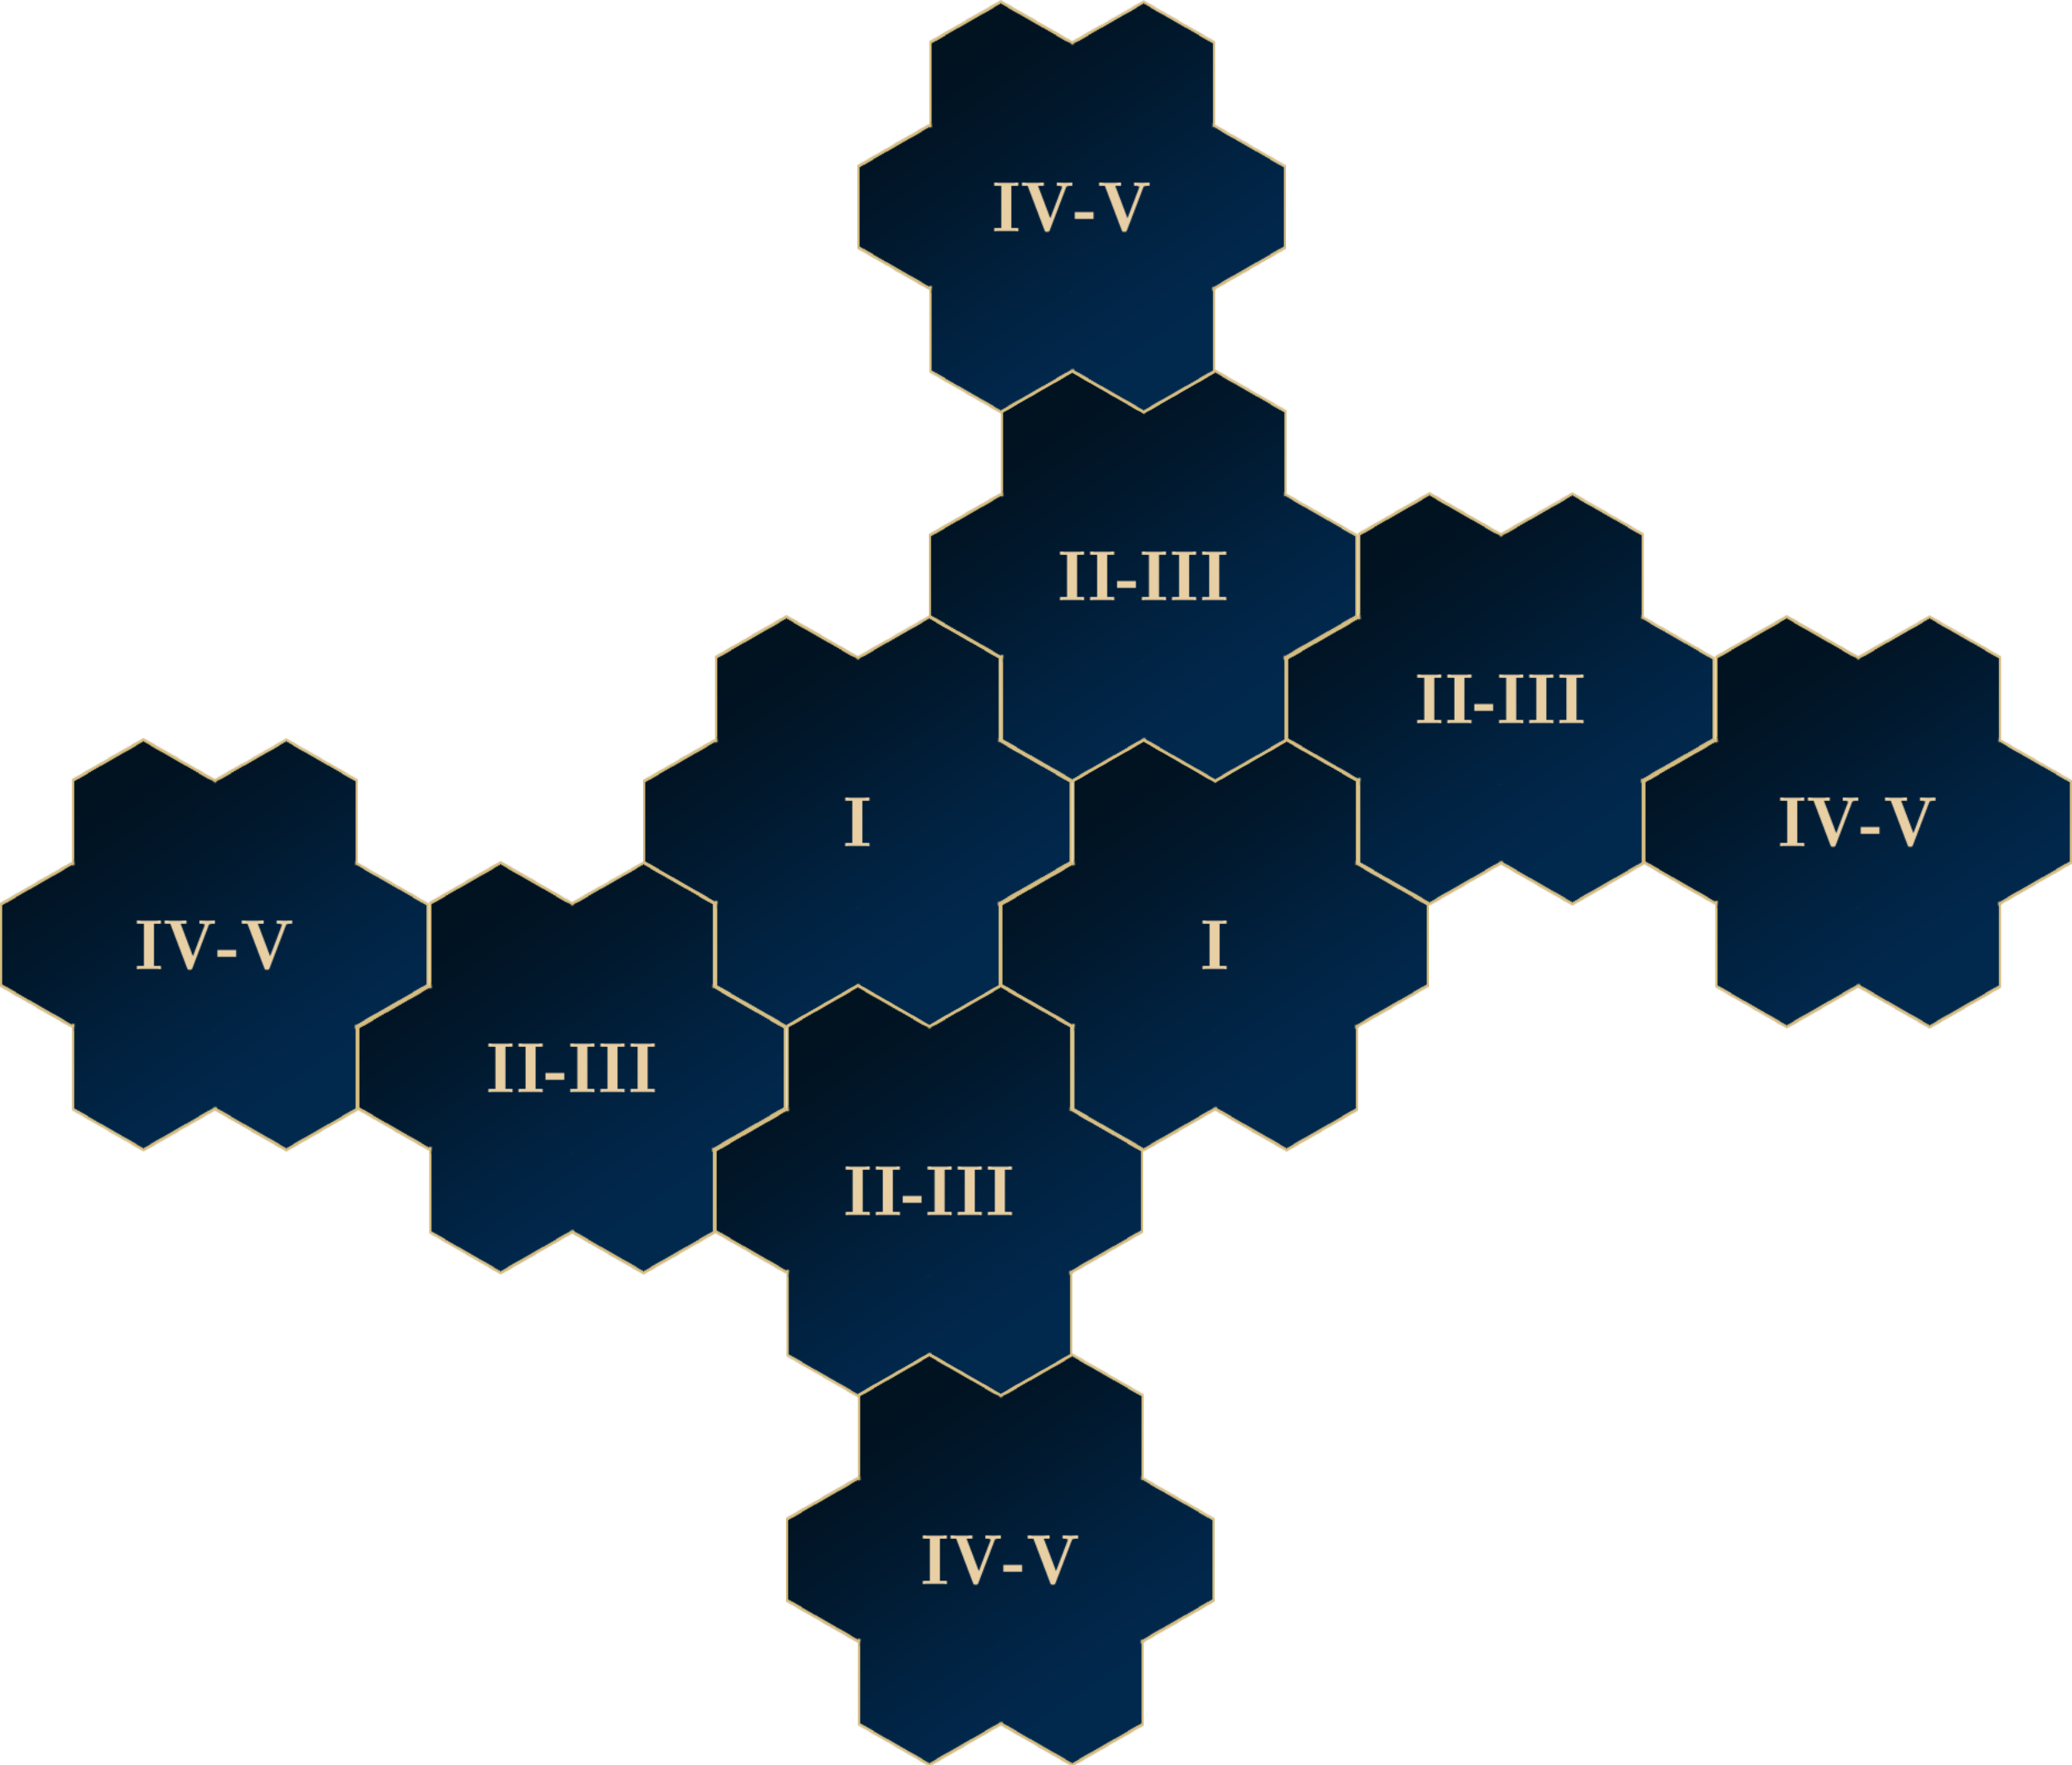
\includegraphics[width=0.6\paperwidth]{\_assets/maps/sentinels.png}
\end{center}

\footnotetext[1]{Always 1 unit of Azure Dragons (starting units of Boss Army). The rest is random\label{azure}.}
